\documentclass[12pt,a4paper]{report}
\usepackage[latin1]{inputenc}
\usepackage[brazil]{babel}

\usepackage{ucs}
\usepackage{amsmath}
\usepackage{amsfonts}
\usepackage{amssymb}
\usepackage{listings}
\usepackage{color}
\usepackage{graphicx}
\pagestyle{headings}
\author{Frédéric BOLLON}
\title{
    \begin{figure}[htp]
    \centering
    
\includegraphics{doc_fredistrano2.png}
    \caption{Transverse momentum distributions}\label{fig:erptsqfit}
    \end{figure}
    - - -\\Versão 1.0\\- - -\\Documentação\\
}
\begin{document}

\maketitle
\tableofcontents

\chapter{Introdução}
Fredistrano é uma ferramenta para implantação\footnote{Deployment.} para aplicações web PHP.  Fredistrano automatiza a tarefa de exportar o conteúdo dos fontes a partir de um repositório Subversion e sincronizá-los com um diretório de destino.  Várias tarefas corriqueiras também podem ser realizadas diretamente pela ferramenta durante o processo, tais como renomeação de arquivos de configuração ou modificação de permissões...  Fredistrano é uma ferramenta inspirada no projeto Capistrano.\\

De um ponto de vista técnico, esta aplicação está sendo desenvolvida em PHP com o framework CakePHP.  Fredistrano dá suporte tanto a ambientes Windows como Linux.
No caso de Windows, o Fredistrano precisa que o Cygwin esteja instalada para poder usar o comando rsync.\\

Agradecimentos especiais a Aurélien Millet e a euphrate\_ylb por sua contribuição neste projeto.

\chapter{Requisitos}
Fredistrano deve ser instalada em um servidor web Apache, \textbf{independente} se sob um sistema Linux ou Windows.
\paragraph*{Requisitos comuns em qualquer SO}
\begin{itemize}
\item 
Um projeto PHP "versionado" com Subversion
\item 
Um servidor web com suporte a PHP sem modo de segurança (safe\_mode em Off) e com mod\_rewrite habilitado\\\\
\begin{small}\textit{Se o mod\_rewrite não estiver funcionando, você precisará descomentar, no arquivo app/config/core.php\\
      a. Por volta da linha 59: Configure::write('App.baseUrl', env('SCRIPT\_NAME'));\\
      b. Depois, faça um teste acessando sua aplicação como http://www.exemplo.com/meu\_diretorio/index.php/pages para verificar se a instalação está funcionando}\end{small}
\end{itemize}

\paragraph*{Apenas em ambiente Windows}
\begin{itemize}
\item
Para implantação em servidores Windows, você precisa instalar o Cygwin com os pacotes rsync, perl e subversion.

\end{itemize}

\chapter{Instalação}
\begin{itemize}
\item Faça o download da última versão do Fredistrano em\\ http://code.google.com/p/fredistrano/downloads/list
\item Descompacte o arquivo na raiz de seu servidor web ou num diretório de sua escolha \: \\
tar xzvf fredistrano\_x.x.tar.gz \\
\item Adicione permissão de escrita nos diretórios temporários (apenas em servidores Linux).\\
\begin{verbatim}

chmod -R 777 app/tmp/ files/

\end{verbatim}

\item Crie a base de dados com o script SQL presente em \\ /app/config/sql/fredistrano.sql\\
\item Crie os arquivos app/config/config.php e app/config/database.php a partir dos originais config.prd.php e database.prd.php\newpage

\item Modifique o arquivo app/config/database.php de acordo com a configuração de seu banco de dados\\\\por exemplo :\\

%---------------------------------------------------------------
\definecolor{lbcolor}{rgb}{0.9,0.9,0.9}
\lstset{language=Php}
\lstset{commentstyle=\textit}
%\lstset{backgroundcolor=lbcolor,framerulecolor=}
\lstset{backgroundcolor=\color{lbcolor},rulecolor=}
\lstset{literate={<=}{{$\le$}}{2}}
%\color{yellow}

\lstset{literate={=}{{$\leftarrow$}}{1}{<=}{{$\le$}}{2}{&&}{{$\cap$}}{2}}
\begin{lstlisting}[frame=tb]{}
var $default = array(
	'driver' => 'mysql',
	'persistent' => false,
	'host' => 'localhost',
	'login' => 'usermysql',
	'password' => 'password',
	'database' => 'fredistrano'
	'encoding' => 'utf8'
);
\end{lstlisting}
%---------------------------------------------------------------

\item Um usuário "admin" com a senha "pass" terá sido criado pelo script SQL.  Não se esqueça de modificar a senha em Administração/usuários.
Se quiser criar um novo usuário, inclua-o no grupo "admin".
\textbf{Não remova o usuário "admin" se não for criar um novo usuário para o grupo "admin".}

\end{itemize}

\chapter{Usage}
\section{Configurando seu projeto}\label{precimportantes}
Antes de poder implantar seu projeto com Fredistrano, você deve configurá-lo de acordo com as sequintes recomendações :\\
\begin{itemize}
\item Seu projeto deve estar sob controle de versão em um repositório Subversion.\\
\item Se o conteúdo de alguns arquivos precisarem ser diferentes no ambiente de implantação e no de produção, estes arquivos não devem ser adicionados ao Subversion, mas apenas cópias deles com uma extensão como '.dev.xxx' e '.prd.xxx':\\
Por exemplo, se a aplicação precisar que o arquivo database.php, onde os parâmetros de conexão são definidos, você não precisa pôr este arquivo diretamente sob controle de versão.  Ao invés disso, adicione duas cópias do arquivo, uma para cada ambiente, chamadas de database.dev.php e database.prd.php.\\ 
Ao serem transferidos para o ambiente de produção, todos os arquivos com uma extensão 'prd.xxx' (e não os 'dev.xxx') serão renomeados para apenas '.xxx'.
\item Um diretório ".fredistrano" deve ser criado na raiz da aplicação.  Neste diretório você deve criar um arquivo chamado "deploy.php".  Este arquivo contém parâmetros específicos de implantação de sua aplicação, tais como uma lista de arquivos e pastas que não devem ser sincronizados, uma lista de diretórios que devem ter permissão de escrita, e etc.  Note que este arquivo não será sincronizado para o ambiente de produção.  Veja um exemplo de um arquivo deploy.php :\\

%---------------------------------------------------------------
\definecolor{lbcolor}{rgb}{0.9,0.9,0.9}
\lstset{language=Php}
\lstset{breaklines=true}
\lstset{tabsize=2}
\lstset{morecomment=[l]{//}}
\lstset{commentstyle=\textit}
\lstset{backgroundcolor=\color{lbcolor},rulecolor=}
\begin{lstlisting}[frame=tb]{}
	<?php
	 class DEPLOY_CONFIG {

		// Opções padrão de implantação para o projeto atual
		// estas opções podem ser modificadas durante o processo de implantação no modo padrão
		// no modo rápido estas opções serão usadas
	 	var $options = array(
	 		'export' 		=> array(),
	 		'synchronize'	=> array(
	 		 	'runBeforeScript'		=> 	false, 		//habilita scripts personalizados antes da implantação
	 			'backup'				=> 	false 		//habilita a funcionalidade de backup
	 		),
	 		'finalize'		=> array(
		 		'renamePrdFile' 		=> 	false,		//habilita renomeação de arquivos .prd.xxx
				'changeFileMode' 		=> 	false,		//habilita modo de sobrescrita de arquivos
				'giveWriteMode'			=> 	false,		//habilita modo de atualização de escrita nos diretórios definidos em $writable (neste mesmo arquivo)
	 			'runAfterScript'		=> 	false		//habilita scripts personalizados ao final da implantação
	 		)
	 	);

	 	// caminho de seus scripts personalizados a serem executados ao início/final da tarefa de implantação
		// se seus scripts estiverem localizados em um diretório chamado ".fredistrano" na raiz de seu projeto, inclua apenas o nome dos arquivos de script a serem executados
	 	var $scripts = array(
	 		'before' 	=>		'/path/to/file', 
	 		'after' 	=>		'/path/to/file' 
	 	);

		// lista dfe diretórios e arquivos a serem excluídos durante o tarefa de implantação no ambiente de produção
		var $exclude = array (
			'/app/tmp/logs/*',
			'/app/tmp/sessions/*',
			'/app/tmp/tests/*',
			'/app/config/database.php',
			'/app/config/config.php',
			'/app/webroot/files/*',
			'/files/logs/*',
			'/files/tmp/*'
		);

		// lista de diretórios os quais terão permissão de escrita ao final da tarefa de implantação
		// log, cache, diretórios de upload, etc...
		var $writable = array (
			'/app/tmp',
			'/files/backup',
			'/files/logs'
		);

	 }// DEPLOY_CONFIG
	?>
\end{lstlisting}
%---------------------------------------------------------------

\end{itemize}
\newpage

\section{Etapas de implantação}

\subsection{Adicionando um novo projeto}

Para implantar uma aplicação web PHP com o Fredistrano, o primeiro passo é criar um novo projeto.\\

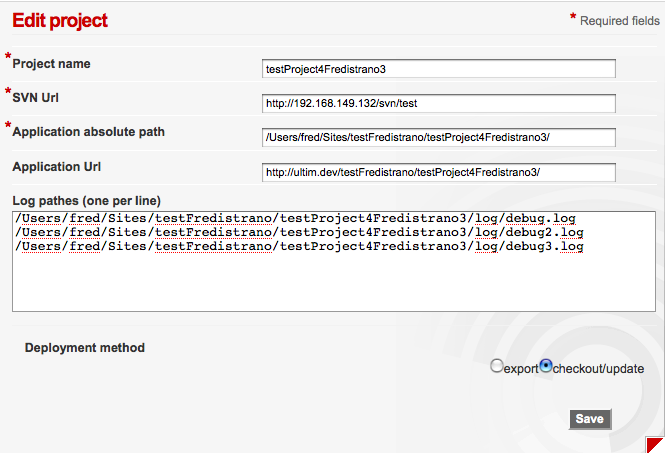
\includegraphics[width=1\textwidth]{doc_fredistrano1.png} 

\begin{enumerate}
\item Clique em "Projects" (parte de cima da tela)
\item Clique no link "Adicionar um novo projeto"
\item Preencha o formulário seguinte:\\

\begin{list}{- Campo:}{}
\item \textbf{"Nome do projeto"} : É usado para identificar o projeto.  O nome do projeto também é usado como nome do diretório de cópia temporário durante a tarefa de implantação.  Não utilize caracteres especiais.
\item \textbf{"URL SVN"} :  URL do repositório do Subversion do projeto a ser implantado (p.ex. : "http://svn.meudominio.com/meuProjeto/trunk").
\item \textbf{"URL da aplicação"} : Não é usada pelo Fredistrano.  Serve apenas como um lembrete :-).
\item \textbf{"Caminho absoluto da aplicação"} :  Caminho absoluto do diretório que deve conter a aplicação no ambiente de produção\\Um exemplo, considerando um servidor de produção Windows, poderia ser : D:\textbackslash www\textbackslash html\textbackslash meuProjeto \\E em um servidor Linux, poderia ser : /var/www/html/meuProjeto ou /home/meuUsuario/meuDominio.
\item \textbf{"Caminho dos arquivos de log"} : Caminho dos arquivos que você pode querer consultar para examinar arquivos de log, um por linha.
\item \textbf{"Método de implantação"} : \textbf{Checkout/update:} o método mais rápido.  Usa o comando "svn checkout" para a primeira implantação, e então o comando "svn update" nas seguintes para obter apenas os arquivos modificados.  \textbf{Export:} mais lento, pois executa o comando "svn export", que sincroniza todo o projeto no repositório a cada implantação.  Entretanto, algumas vezes é necessário usar este método, por exemplo, se você não tem permissão suficientes no repositório Subversion para executar o comando checkout.

\end{list}
\end{enumerate}

\subsection{Implantação de um projeto}
\begin{enumerate}
\item Exiba os detalhes do projeto a ser implantado.
\item Clique em "Implantar projeto".
\item Especifique o número de revisão desejado.  Se ficar em branco, o Fredistrano irá fazer o checkout da última revisão do repositório.
\item No caso de um projeto Subversion protegido por login/senha, você pode especificar suas credenciais neste passo.  Se todos os seus projetos estiverem usando as mesmas credenciais, você pode especificá-las no arquivo \textit{app/config/config.php}.
\item Clique em "Passo 1 exportar SVN".  O comando "svn export" é executado e o resultado é mostrado no console na parte de baixo da tela (\textit{output console}) "Fredistrano/files/tmp/nomedoprojeto/tempDir".
\item For the next step, if "simulate" is checked, the rsync command will only be simualted and its  result may be seen in the output console.
\item Clique em "Passo 2 sincronizar".
\item Um backup é executado em "Fredistrano/files/backup/nomedoprojeto".  O comando rsync é executado entre "Fredistrano/files/tmp/nomedoprojeto/tempDir" e "nomedoprojeto".
\item Finalmente, como último passo, três opções que podem ser sobrescritas: 1) renomeação dos arquivos '.prd.', 2) modificação das permissões de arquivos e diretórios e 3) definição de permissões de escrita em pastas especiais.  Os valores iniciais desses itens dependem do conteúdo de seu arquivo config.php.
\item Clique em "Passo 3 finalizar" e pronto!
\end{enumerate}

\subsection{Implantação de projeto em modo rápido}
\begin{enumerate}
\item Exiba os detalhes do projeto a ser implantado.
\item Clique no link "trocar o modo de implantação" para mudar o botão "Implantação" para "Implantação rápida"
\item Todos os passos serão executados com as opções do modo padrão (renomeação de arquivos .prd, definição de permissões apenas nos arquivos modificados, adicionando permissão de escrita). 
\end{enumerate}

\section{Logs de implantação}
Você pode acessar o histórico de implantação a partir da página de detalhes de cada projeto ao clicar no link "ver histórico de implantação".  Um feed RSS do histórico de implantação está disponível no menu desta página.  É possível desabilitar feeds RSS no arquivo de configuração /app/config/config.php 

\section{Visualizador de logs}
Clique na aba "Logs" para usar o visualizador de logs.  Com este recurso você pode exibir o conteúdo dos arquivos de log definidos nos detalhes do projeto.

\section{Dicas}
\subsection{Dicas comuns a todos os tipos de projeto} % (fold)
\begin{list}{-}{}
\item \textbf{Exemplo de script "beforeScript"}\\
Este script possibilita substituir arquivos .htaccess de um projeto por outros .htaccess para redirecionar os visitantes momentaneamente a uma página temporária durante a tarefa de sincronização.  O arquivo .htaccess temporário e a página que serão usadas para redirecionamento estão presentes no diretório .fredistrano na raiz do projeto.

	\definecolor{lbcolor}{rgb}{0.9,0.9,0.9}
	\lstset{language=bash}
	\lstset{breaklines=true}
	\lstset{tabsize=1}
	\lstset{backgroundcolor=\color{lbcolor},rulecolor=}
	\begin{lstlisting}[frame=tb]{}
	#!/bin/sh

	PATHTMP=/Path/on/production/server/fredistrano/files/tmp/meuProjeto/tmpDir
	PATHPRD=/Path/on/production/server/meuProjeto

	# copia o arquivo .htaccess temporário para o lugar correto
	cp -vf ${PATHTMP}/.fredistrano/.htaccess ${PATHPRD}/.htaccess
	# copia a página de redirecionamento temporário para o lugar correto
	cp -vf ${PATHTMP}/.fredistrano/302.html ${PATHPRD}/302.html
	\end{lstlisting}

\item \textbf{Exemplo de script "afterScript"}\\
Este script irá mudar um valor no arquivo.  Neste exemplo ele irá modificar o o modo de debug para 0 no arquivo app/config/core.php.  Ele também irá restaurar o arquivo .htaccess que foi substituído por um arquivo temporário durante a tarefa de implantação e vai remover o arquivo de redirecionamento (veja o exemplo anterior do script "beforeScript")
	\definecolor{lbcolor}{rgb}{0.9,0.9,0.9}
	\lstset{language=bash}
	\lstset{breaklines=true}
	\lstset{tabsize=1}
	\lstset{backgroundcolor=\color{lbcolor},rulecolor=}
	\begin{lstlisting}[frame=tb]{}
	#!/bin/sh
	# modifica o modo debug para 0 no arquivo app/config/core.php
	PATHTMP=/Path/on/production/server/fredistrano/files/tmp/meuProjeto/tmpDir
	PATHPRD=/Path/on/production/server/myproject

	sed -i.bak "s/\('debug',\)[ ]*[12]/\1 0/g" ${PATHPRD}/app/config/core.php

	# substitui o arquivo .htaccess temporário
	cp -vf ${PATHTMP}/.htaccess ${PATHPRD}/.htaccess

	# remove a página temporária de redirecionamento
	rm -vf ${PATHPRD}/302.html
	# remove a versão antiga de app/config/core.bak
	rm -vf ${PATHPRD}/app/config/core.php.bak
	\end{lstlisting}


\end{list}
% subsection commun_Ã _tous_type_de_projet (end)

\subsection{Dicas específicas para projetos CakePHP} % (fold)
\begin{list}{-}{}
	\item \textbf{Limpeza de cache:} Para esvaziar o cache automaticamente durante cada implantação, você precisa versionar os diretórios app/tmp/cache/models, app/tmp/cache/persistent e app/tmp/cache/views e ignore seus conteúdos.  Desta forma, durante a etapa de sincronização, estes diretórios serão mantidos vazios também no servidor de produção..\\
	Para ignorar o conteúdo destes diretórios eu utilizo o seguinte comando na raiz da cópia de trabalho:
	\definecolor{lbcolor}{rgb}{0.9,0.9,0.9}
	\lstset{language=bash}
	\lstset{breaklines=true}
	\lstset{tabsize=1}
	\lstset{backgroundcolor=\color{lbcolor},rulecolor=}
	\begin{lstlisting}[frame=tb]{}
	svn propset svn:ignore "*" app/tmp/cache/models/ app/tmp/cache/persistent/ app/tmp/cache/views/ app/tmp/logs/ app/tmp/sessions/ app/tmp/tests/
	\end{lstlisting}
\end{list}
% subsection spécifiques_aux_projets_basés_sur_cakephp (end)




\chapter{Links relacionados}
\begin{itemize}
\item Um exemplo de servidor web de hospedagem que satisfaz aos requisitos do Fredistrano \\ http://www.fbollon.net/node/12 \\
\item Uma rápida explicação de como usar o Subversion \\ http://www.fbollon.net/node/65 \\
\item O fórum de suporte oficial do Fredistrano \\ http://groups.google.com/group/fredistrano-discuss
\end{itemize}


\end{document}
